% LaTeX Präsentationsvorlage (2013) der TU Graz, rev12, 2013/01/31
\documentclass{beamer}
%\documentclass[aspectratio=169]{beamer}
% \usetheme{tugraz2013}
% \usetheme[notes]{tugraz2013}
\usetheme[minimal]{tugraz2013}
\usepackage[utf8]{inputenc}
\usepackage[american]{babel}
\usepackage{color, colortbl}
\usepackage{listings}
\usepackage{tikz}
\usepackage{alltt}
\usepackage{graphicx}
\usepackage{adjustbox}

\usepackage{amssymb}% http://ctan.org/pkg/amssymb
\usepackage{pifont}% http://ctan.org/pkg/pifont
\newcommand{\cmark}{\ding{51}}%
\newcommand{\xmark}{\ding{55}}%

%\usepackage{ulem}
\usetikzlibrary{calc,trees,positioning,arrows,chains,shapes.geometric,decorations.pathreplacing,decorations.pathmorphing,shapes,matrix,shapes.symbols}
%\newcommand{\iocosymbol}{\ensuremath{\mbox{\it{ioco}}}\xspace}
\makeatletter
\def\cellcolor{{\ifnum0=`}\fi\bmr@cellcolor}
\newcommand<>{\bmr@cellcolor}{%
    \alt#1%
        {\global\let\CT@do@color\CT@@do@color\@ifnextchar[\CT@rowa\CT@rowb}% 
        {\ifnum0=`{\fi}\@gooble@cellcolor}% 
}

\newcommand{\@gooble@cellcolor}[2][]{\@gooble@cellcolor@}
\newcommand{\@gooble@cellcolor@}[1][]{\@gooble@cellcolor@@}
\newcommand{\@gooble@cellcolor@@}[1][]{\ignorespaces}

\def\intf{Spec}
\def\tc{t}
\def\verdict{x_{v}}
\def\pass{\textbf{pass}}
\def\fail{\textbf{fail}}


\makeatother

% This sets a new round of anchors at a specified multiple of the current ones
\def\pgf@sh@@knotanchor#1#2{%
  \anchor{#2 north west}{%
    \csname pgf@anchor@knot #1@north west\endcsname%
    \pgf@x=#2\pgf@x%
    \pgf@y=#2\pgf@y%
  }%
  \anchor{#2 north east}{%
    \csname pgf@anchor@knot #1@north east\endcsname%
    \pgf@x=#2\pgf@x%
    \pgf@y=#2\pgf@y%
  }%
  \anchor{#2 south west}{%
    \csname pgf@anchor@knot #1@south west\endcsname%
    \pgf@x=#2\pgf@x%
    \pgf@y=#2\pgf@y%
  }%
  \anchor{#2 south east}{%
    \csname pgf@anchor@knot #1@south east\endcsname%
    \pgf@x=#2\pgf@x%
    \pgf@y=#2\pgf@y%
  }%
  \anchor{#2 north}{%
    \csname pgf@anchor@knot #1@north\endcsname%
    \pgf@x=#2\pgf@x%
    \pgf@y=#2\pgf@y%
  }%
  \anchor{#2 east}{%
    \csname pgf@anchor@knot #1@east\endcsname%
    \pgf@x=#2\pgf@x%
    \pgf@y=#2\pgf@y%
  }%
  \anchor{#2 west}{%
    \csname pgf@anchor@knot #1@west\endcsname%
    \pgf@x=#2\pgf@x%
    \pgf@y=#2\pgf@y%
  }%
  \anchor{#2 south}{%
    \csname pgf@anchor@knot #1@south\endcsname%
    \pgf@x=#2\pgf@x%
    \pgf@y=#2\pgf@y%
  }%
}
% this defines the new node shape, inheriting most from the circle shape
\pgfdeclareshape{knot crossing}
{
  \inheritsavedanchors[from=circle] % this is nearly a circle
  \inheritanchorborder[from=circle]
  \inheritanchor[from=circle]{north}
  \inheritanchor[from=circle]{north west}
  \inheritanchor[from=circle]{north east}
  \inheritanchor[from=circle]{center}
  \inheritanchor[from=circle]{west}
  \inheritanchor[from=circle]{east}
  \inheritanchor[from=circle]{mid}
  \inheritanchor[from=circle]{mid west}
  \inheritanchor[from=circle]{mid east}
  \inheritanchor[from=circle]{base}
  \inheritanchor[from=circle]{base west}
  \inheritanchor[from=circle]{base east}
  \inheritanchor[from=circle]{south}
  \inheritanchor[from=circle]{south west}
  \inheritanchor[from=circle]{south east}
  \inheritanchorborder[from=circle]
  \pgf@sh@@knotanchor{crossing}{2}
  \pgf@sh@@knotanchor{crossing}{3}
  \pgf@sh@@knotanchor{crossing}{4}
  \pgf@sh@@knotanchor{crossing}{8}
  \pgf@sh@@knotanchor{crossing}{16}
  \pgf@sh@@knotanchor{crossing}{32}
  \backgroundpath{
    \pgfutil@tempdima=\radius%
    \pgfmathsetlength{\pgf@xb}{\pgfkeysvalueof{/pgf/outer xsep}}%
    \pgfmathsetlength{\pgf@yb}{\pgfkeysvalueof{/pgf/outer ysep}}%
    \ifdim\pgf@xb<\pgf@yb%
      \advance\pgfutil@tempdima by-\pgf@yb%
    \else%
      \advance\pgfutil@tempdima by-\pgf@xb%
    \fi%
  }
}

\lstdefinelanguage{scala}{
  morekeywords={abstract,case,catch,class,def,%
    do,else,extends,false,final,finally,%
    for,if,implicit,import,match,mixin,%
    new,null,object,override,package,%
    private,protected,requires,return,sealed,%
    super,this,throw,trait,true,try,%
    type,val,var,while,with,yield},
  otherkeywords={=>,<-,<\%,<:,>:,\#,@},
  sensitive=true,
  morecomment=[l]{//},
  morecomment=[n]{/*}{*/},
  morestring=[b]",
  morestring=[b]',
  morestring=[b]"""
}



\lstdefinelanguage{assumeguarantee} {
  alsoletter={ ; , [] , |[ , ]|, 0, 1, 2, 3, 4, 5, 6, 7, 8, 9 },
  morekeywords={and, not, assume, guarantee},
   emph={SmallInt, TimeSteps, int, Int, bool, AlarmSystem},
   emphstyle=\color{brown},
%   emph={true, false, and, not, of, len, //, hd, tl },
%   emphstyle=\color{black},
%   emph={ ; , [] },
%   emphstyle=\color{red},
   sensitive=true,
%   morecomment=[s]{/*}{*/},
   comment=[l]{\#},
   showspaces=false,
   showstringspaces=false,
   numbers=left,
   numbersep=5pt,
   numberstyle=\tiny,
%   showtabs=true,
   tabsize=2,
   escapeinside={@}{@},
   framexleftmargin=9pt,
  }

%\newcommand{\defeq}{\stackrel{def}{=}}
\newcommand{\defeq}{=_{def}}
\tikzstyle{rail}=[ultra thick]
\tikzstyle{movement}=[green!50!black,line width=5\pgflinewidth]
\tikzstyle{marked}=[blue!50!black,line width=5\pgflinewidth]
\tikzstyle{ttx}=[rectangle,draw,fill=green!30, minimum width=1cm, minimum height=0.6cm]
\tikzstyle{ter}=[rectangle,draw,fill=blue!30,minimum width=1cm, minimum height=0.6cm]
\newcommand*{\railWEend}{+ (-.3,0) -- + (.3,0) + (0,0)}
\newcommand*{\railNSend}{+ (0,.3) -- + (0,-.3) + (0,0)}
\newcommand*{\signalLeft}[1]{+ (0,-.3) -- + (0,1.3) node[anchor=east, midway] {\Large #1} node[anchor=east, at end, draw, regular polygon, regular polygon sides=3,shape border rotate=270] {}+ (0,0)}
\newcommand*{\signalRight}[1]{+ (0,-.3) -- + (0,1.3) node[anchor=west, midway] {\Large #1}node[anchor=west, at end, draw, regular polygon, regular polygon sides=3,shape border rotate=90] {}+ (0,0)}




%% Titelblatt-Einstellungen
\title{Incremental Model-based (Mutation) Testing}
\author{Stefan Tiran}
%\today
% \date{Graz, XX. Dezember 2010}		% \today für heutiges Datum verwenden
%\date{\today}
\date{Graz, 2015-04-15}
%\date{Graz, 2013-06-20}		% \today für heutiges Datum verwenden

% \institutelogo{kurz.pdf}
%\additionallogo{institutslogo.pdf}
\institute[TU Graz / AIT]{Graz~University of Technology, Institute for Software Technology and Austrian Institute of Technology\\Supervisor: Bernhard Aichernig}
%\instituteurl{www.tugraz.at}
% \institutelogo{kurz.pdf}
%\additionallogo{institutslogo.pdf}
\additionallogo{ait_logo.jpg}
\additionallogoB{momut1.png}
\additionallogoC{CRYSTAL.png}

%%%%%%%%%%%%%%%%%%%%%%%%%%%%%%%%%%%%%%%%%%%%%%%%%%%%%%%%%%%%%%%%%%%%%%%%%%%%
\begin{document}
%%%%%%%%%%%%%%%%%%%%%%%%%%%%%%%%%%%%%%%%%%%%%%%%%%%%%%%%%%%%%%%%%%%%%%%%%%%%
\titleframe

\section{Introduction}

\begin{frame}
  \frametitle{Research Question}
  Challenge: complexity of industrial systems
  \vspace{.25cm}
  \newline
  ``How can the {\color{blue} knowledge of the structure} of a test model {\color{blue} improve the
  performance} in model-based testing?''
  \pause
  \vspace{.25cm}
  \newline

  Sub projects:
  \begin{enumerate}
    \item Incremental reachability analysis
    \item Modeling in a manner that facilitates incremental test-case generation
    \item Synchronous vs. asynchronous modeling
  \end{enumerate}
\end{frame}

\begin{frame}
  \frametitle{Modeling language: ``Requirement Interfaces''}
  \vspace{-.5cm}
  \begin{figure}
  \scalebox{0.4}{ \input verview.pdf_t }
  \end{figure}
  \scalebox{0.55}{
  \begin{minipage}[H]{1.8\textwidth}
  Source: Bernhard K. Aichernig, Klaus Hörmaier, Florian Lorber, Dejan Nickovic, and Stefan Tiran. Require, Test and Trace IT. In FMICS'15, Oslo, Norway, June 22\textsuperscript{nd}–23\textsuperscript{rd} 2015
  \end{minipage}
  }
\end{frame}

\begin{frame}
  \frametitle{Modeling language: ``Requirement Interfaces'' (cont.)}
  \scalebox{0.9}{
\begin{minipage}[T]{1.11\textwidth}

  \begin{itemize}
    \item Synchronous steps, in which all variables are updated
    \item Model consists of contracts (assume - guarantee
pairs)
    \item Each contract constraints the behavior of the modeled system
    \item Step-relation and reachability encoded as SMT problem
    \item Example (Abstract buffer)
    \begin{itemize}
      \item Requirement R1: ``{\sf enq} triggers an enqueue operation when the buffer is not full.''
      \item Contract: \texttt{\{R1\} {\color{blue} assume} enq' and not deq' and k < N  {\color{violet} guarantee} k' = k + 1}
    \end{itemize}
  \end{itemize}
  \end{minipage}}
\end{frame}

\begin{frame}
  \frametitle{Incremental Reachability Analysis}
  \framesubtitle{The Approach}
 % \vspace{-1cm}

  \begin{minipage}[T]{0.45\textwidth}

  \begin{figure}
    \resizebox{\textwidth}{!}{
  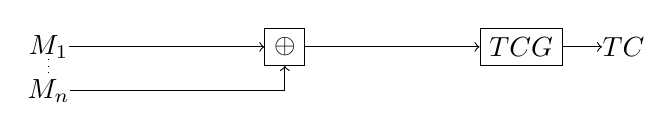
\begin{tikzpicture}[node distance=3cm]
    \tikzstyle{fun}=[rectangle,draw]
    \tikzstyle{inv}=[inner sep=0]
    \node[inv] (Ab) {$M_1$} ;
    \node[inv] (Ac) [below =.25cm of Ab] {$M_n$} ;
    \node[fun] (conj) [right of=Ab] {$\oplus$} ;
    \node[fun] (TC) [right of=conj] {$TCG$} ;
    \node[inv] (result) [right =0.5 cm of TC] {$TC$};
    \node[inv] (h1) [right of=Ac] {} ;
    \draw[dotted] (Ab) -- (Ac) ;
    \draw[->] (Ab) -- (conj) ;
    \draw[->] (Ac) -| (conj) ;
    \draw[->] (conj) -- (TC) ;
    \draw[->] (TC) -- (result) ;
  \end{tikzpicture}
}
{\tiny monolithic}
\label{fig:overview_mono_tcg}
\end{figure}

\begin{figure}
  \resizebox{\textwidth}{!}{
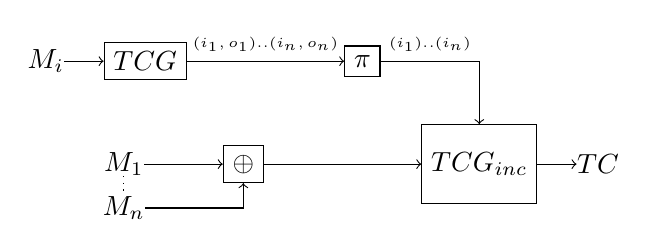
\begin{tikzpicture}[node distance=3cm]
 \tikzstyle{fun}=[rectangle,draw]
 \tikzstyle{inv}=[inner sep=0]
  \node[inv] (Aa) {$M_i$} ;
  \node[inv] (Ab) [below right=1cm and 0.5 cm of Aa] {$M_1$} ;
  \node[inv] (Ac) [below =.25cm of Ab] {$M_n$} ;
  \node[fun] (conj) [right =1 cm of Ab] {$\oplus$} ;
  \node[fun] (TC) [right= 0.5cm of Aa] {$TCG$} ;
  \node[fun] (proj) [right=2 cm of TC] {$\pi$} ;
  %\node[inv] (h1) [right =2.35 cm of Ac] {} ;
  %\node[inv] (h2) [right of=proj] {} ;
  \node[fun, minimum height=1cm] (TCinc) [right= 2cm of conj] {$TCG_{inc}$} ;
  \node[inv] (result) [right =0.5 cm of TCinc] {$TC$};
\draw[dotted] (Ab) -- (Ac) ;
\draw[->] (Aa) -- (TC) ;
\draw[->] (TC) -- (proj) node[anchor=south, midway] {\tiny $(i_1,o_1) .. (i_n,o_n)$};
\draw[->] (proj) -| (TCinc) node[anchor=south,near start] {\tiny $(i_1) .. (i_n)$}    ;
\draw[->] (TCinc) -- (result) ;
%\draw[->] (Aa) -- (conj) ;
       \draw[->] (Ab) -- (conj) ;
       \draw[->] (Ac) -| (conj) ;
       \draw[->] (conj) -- (TCinc) ;
     \end{tikzpicture}}
{\tiny incremental}
\label{fig:overview_inc_tcg}
\end{figure}
\end{minipage}
\begin{minipage}[T]{0.45\textwidth}
\scalebox{0.7}{
\begin{minipage}[T]{1.5\textwidth}
  \begin{itemize}
    \item Search on partial models instead of one monolithic model
	\item Benefit from structure given by
	\begin{itemize}
	  \item multiple view-point modeling
	  \item object-orientation
	\end{itemize}
	\item Incrementally extending test-case
	\begin{itemize}
	  \item Complete test-oracle
	  \item Catch errors from other view-points / components
	\end{itemize}
  \end{itemize}
\end{minipage}
}
\end{minipage}
\end{frame}

\begin{frame}
  \frametitle{Incremental Reachability Analysis}
  \framesubtitle{First Results}
  \begin{itemize}
    \item Two case studies
    \begin{itemize}
       \item ECU of a wheel-loader 
       \item Interlocking system
    \end{itemize}
    \item Series of test models (different configurations)
    \item Proof of concept: Just one test purpose
    \item Increased scalability
    \begin{itemize}
      \item Wheel-loader: $> 9 h$ vs. $\sim 8 s$
      \item Interlocking: $> 1 h$ vs. $\sim 8 min$
    \end{itemize}
    
  \end{itemize}
\end{frame}


% \begin{frame}
  % \frametitle{Modeling for incremental test-case generation}
  % \begin{itemize}
    % \item ``How to preserve object-oriented structure?''
    % \item Requirement interfaces lack notion of objects or components
    % \item Use of Scala to extend modeling language
    % \item Proposed concept: ``parametrized contracts''
    % \item Already used in order to model interlocking system
    % \item Also interesting for asynchronous models
  % \end{itemize}
% \end{frame}

% \begin{frame}
  % \frametitle{Synchronous vs. asynchronous modeling}
  % \begin{itemize}
    % \item Incremental approach based on Krenn et al. 2013\textsuperscript{1}
    % \item Originally proposed for networks of timed automata (asynchronous)
    % \item Asynchronous styles facilitate modeling
    % \item Synchronous styles facilitate reachability analysis
    % \item Upcoming case study will include communication protocol
  % \end{itemize}
    % \scalebox{0.55}{
  % \begin{minipage}[H]{1.8\textwidth}
  % \textsuperscript{1}Willibald Krenn, Dejan Nickovic, and Loredana Tec. Incremental language
% inclusion checking for networks of timed automata. In FORMATS, volume 8053 of
% LNCS, pages 152–-167. Springer, 2013.
  % \end{minipage}}
% \end{frame}

\begin{frame}
  \frametitle{Next steps}
    \scalebox{0.8}{
\begin{minipage}[T]{1.25\textwidth}
  \begin{itemize}
    \item Modeling for incremental test-case generation
    \begin{itemize}
      \item ``How to preserve object-oriented structure?''
      \item Use of Scala to extend modeling language
      \item Proposed concept: ``parametrized contracts''
    \end{itemize}
    \item Back to asynchronous models
    \begin{itemize}
      \item Incremental approach based on Krenn et al. 2013\textsuperscript{1}
      \item Originally proposed for networks of timed automata (asynchronous)
      \item Synchronous styles facilitate reachability analysis
      \item Asynchronous styles facilitate modeling
    \end{itemize}
    \end{itemize}
    \end{minipage}}
    \scalebox{0.55}{
     \begin{minipage}[H]{1.8\textwidth}
     \vspace{.5cm}
   \textsuperscript{1}Willibald Krenn, Dejan Nickovic, and Loredana Tec. Incremental language
 inclusion checking for networks of timed automata. In FORMATS, vol. 8053 of
 LNCS, pages 152–-167. Springer, 2013.
   \end{minipage}}
\end{frame}

\begin{frame}
  \frametitle{Conclusion}
  \begin{itemize}
    \item Technique implemented for synchronous models
    \item Evaluation based on two industrial sized case studies
    \item Enormous performance gains (from hours to minutes / seconds) 
    \item Further automation needed
    \begin{itemize}
      \item Automatically create partial model
      \item Back-tracking
    \end{itemize}
    \item Upcoming case study: communication protocol for railway systems
  \end{itemize}
\end{frame}



\begin{frame}
  \frametitle{Publications}
    \scalebox{0.55}{
  \begin{minipage}[H]{1.8\textwidth}
  \begin{enumerate}
    %\item Bernhard K. Aichernig, Dejan Nickovic, and \textbf{Stefan Tiran}. Scalable incremental test-case generation from large behavior models. In TAP'15, submitted
    \item Bernhard K. Aichernig, Klaus Hörmaier, Florian Lorber, Dejan Nickovic, and \textbf{Stefan Tiran}. Require, Test and Trace IT. In FMICS'15, Oslo, Norway, June 22\textsuperscript{nd}–23\textsuperscript{rd} 2015. In press.
    \item Bernhard K. Aichernig, Harald Brandl, Elisabeth Jöbstl, Willibald Krenn, Rupert Schlick, and \textbf{Stefan Tiran}. Killing strategies for model-based mutation testing. STVR journal, 2014.
    \item Bernhard K. Aichernig, Elisabeth Jöbstl, and \textbf{Stefan Tiran}. Model-based mutation testing via symbolic refinement checking. Science of Computer Programming, 97, Part 4(0):383--404, 2015. Special Issue: Selected Papers from the 12\textsuperscript{th} International Conference on Quality Software (QSIC 2012).
    \item Bernhard K. Aichernig, Klaus Hörmaier, Florian Lorber, Dejan Ničković, Rupert Schlick, Didier Simoneau, and \textbf{Stefan Tiran}. Integration of Requirements Engineering and Test-Case Generation via OSLC. In QSIC '14: Proceedings of the 2014 14\textsuperscript{th} International Conference on Quality Software, pages 117--126, Dallas, USA, 2014. IEEE Computer Society.
    \item Bernhard K. Aichernig, Florian Lorber, and \textbf{Stefan Tiran}. Formal test-driven development with verified test cases. In MODELSWARD'14, pages 626–-635, Lisbon, January 2014. SCITEPRESS.
    \item Bernhard K. Aichernig, Florian Lukas Lorber, and \textbf{Stefan Tiran}. Integrating model-based testing and analysis tools via test case exchange. In IEEE Computer Society, editor, Proceedings of the 2012 6\textsuperscript{th} International Symposium on Theoretical Aspects of Software Engineering, pages 119--126. IEEE Computer Society, July 2012.
  \end{enumerate}
  \end{minipage}}
\end{frame}

\section{Backup Slides}

\begin{frame}
  \frametitle{Wheel loader case study - results}
  \vspace{-1cm}
  \small Test goal: reach ``STOP'' state
  %\begin{minipage}[T]{\linewidth}
  \begin{table}  
  \resizebox{0.7\textwidth}{!}{

  \centering
 \begin{tabular}{c c c r r r r r}
   \multicolumn{3}{c}{Configuration} &  & &  & & \\
   K & M & N & Depth & $vars$ & $t_{incremental}$ &$t_{monolithic}$\\
\hline 
 4 & 3 & 5 & 41 &  861 & 3.6 & 16.8 \\
 4 & 3 & 6 & 45 &  945 & 3.4 & 47.7 \\
 4 & 4 & 5 & 46 & 966 & 2.8 & 31.9 \\
 4 & 3 & 7 & 49 & 1029 & 4.6 & 139.1 \\
 4 & 4 & 6 & 50 & 1050 & 3.9 & 45.3 \\
 4 & 5 & 5 & 51 & 1071 & 4.9 & 47.5 \\
 4 & 3 & 8 & 53 & 1113 & 4.8 & 52.2 \\
 4 & 4 & 7 & 54 & 1134 & 4.6 & 53.7 \\
 4 & 5 & 6 & 55 & 1155 & 4.8 & 252.4 \\
 4 & 4 & 8 & 58 & 1218 & 7.3 & 135.4 \\
 4 & 5 & 7 & 59 & 1239 & 7.8 & 33,810.4 \\
\end{tabular}}\\[1ex]
  \caption{Run-times in seconds for the incremental
approach and the monolithic approach for the wheel loader models}
 \label{tab:relab_time_vars}
\vspace{-.5cm}

%\end{minipage}
\end{table}
\end{frame}

\begin{frame}
  \frametitle{Interlocking Case Study - Results}
\begin{table}
  \centering
  \resizebox{0.7\textwidth}{!}{
 \begin{tabular}{c | r r | r r r}
Model size& \# $vars_{part}$ & \# $vars_{full}$ & $t_{inc}$ & $t_{mono}$\\
\hline 
L & 720 & 1360 & 15.6 & 25.7 \\
XL & 1083 & 2071 & 39.3 & 94.2\\
XXL & 1518 & 2926 & 87.3 & 316.2\\
XXXL & 2025 & 3925 & 173.3 & 413.2\\
XXXXL & 2604 &	5068 & 308.3 &	825.0\\
XXXXXL & 3255 & 6355 & 480.8 & 5476.1\\
\end{tabular}}\\[1ex]
  %\caption{Size of SMT problem in \# vars and run-times in s for finding a trace fulfilling the test-goal \texttt{tr\_13\_state' = 3 and tr\_26\_state' = 3 and TCH\_usage' = 5 and TCSS\_usage' = 5}}
 \label{tab:elektra_runtimes}
\vspace{-.5cm}
\end{table}
\begin{itemize}
%  \item Generating one test-case for an interlocking system
  \item Series of model configurations from L to XXXXXL
  \item Common test goal: Set-up and dissolve two train routes
  \item \# vars determines size of SMT problem
  \item Run-times in seconds
  \item Model size XXXXXL: monolithic: $> 1 h$, incremental: $\sim 8 min$
\end{itemize}
\end{frame}



%%%%%%%%%%%%%%%%%%%%%%%%%%%%%%%%%%%%%%%%%%%%%%%%%%%%%%%%%%%%%%%%%%%%%%%%%%%%
\end{document}
%%%%%%%%%%%%%%%%%%%%%%%%%%%%%%%%%%%%%%%%%%%%%%%%%%%%%%%%%%%%%%%%%%%%%%%%%%%%

%% EOF
